\documentclass{standalone}
\usepackage{mintikz}

\begin{document}
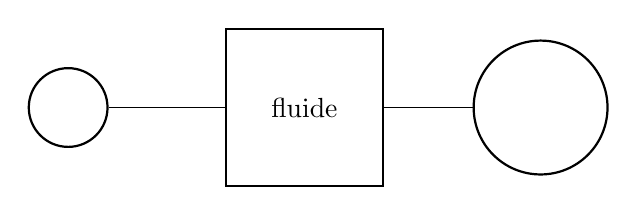
\begin{tikzpicture}
	\def\wdt{3}
	\def\hgt{3}
	\node[draw, thick,
		minimum width=2cm,
		minimum height=2cm,
		anchor=center] (syst) at (0,0)
	{fluide};

	% Source 1
	\node[draw, thick, circle, align=center, minimum width=1cm]
	(S1) at (-\wdt,0)
	{};
	\draw[]
	(S1.east) --
	node[midway, above] {}
	(syst.west);

	% Travail
	\node[draw, thick, circle, align=center, minimum width=1.7cm]
	(W) at (\wdt,0)
	{};
	\draw[]
	(W.west) --
	node[midway, above] {}
	(syst.east);
\end{tikzpicture}
\end{document}
